\section{Methodology}

\begin{frame}
\sectionpage
\end{frame}	

\begin{frame}{Self Organizing Map}

\begin{itemize}
\item {
	Artificial neural network, competitive learning .
}
\item {
Unsupervised learning.
}
\item {
	Maintain the topology of the input.
}
\item {
	Very suitable for visualization of high-dimensional data space.
}
\end{itemize}
\end{frame}

\begin{frame}{Self Organizing Map}
\begin{figure}[htbp]
\centering
\includegraphics[width=8cm]{./figs/SOM1.png}
\caption{Neural network}
\end{figure}

\end{frame}
\begin{frame}{Self Organizing Map}

\begin{itemize}
\item {
	Artificial neural network, competitive learning .
}
\item {
Unsupervised learning.
}
\item {
		Maintain the topology of the input.
}
\item {
	Very suitable for visualization of high-dimensional data space.
}
\end{itemize}
\end{frame}






\begin{frame}{Learning Principle}


\begin{figure}[htbp]
\includegraphics[width=6cm]{./figs/SOM.png}
\caption{ 1. Principle of SOMs. Initial geometry of nodes in $3 \times 2$
rectangular grid is indicated by solid lines connecting the nodes.
}
\end{figure}
\end{frame}



\begin{frame}{Learning Principle}


\begin{figure}[htbp]
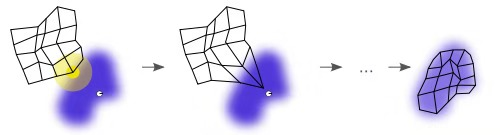
\includegraphics[width=8cm]{./figs/SOM3.jpg}

\caption{The process of SOM}
\end{figure}
\end{frame}





\begin{frame}{Algorithm}
\begin{enumerate}
\item	Select grid structure and initialize the position function $f_0$ of all nodes
\item \textbf{Repeat}
\item	 \quad Calculate \textbf{Euclidean distance} between $X_i$ and all nodes ,and select the node with the smallest distance as best matching unit\,(\textbf{BMU})
\item  \quad Update the position of the nodes in \textbf{BMU’s} neighborhood by the formula:
\begin{equation*}
f_{i+1}(N)=f_i(N)+\tau(d(N,N_p),i)(P-f_i(N))
\end{equation*}
\item \textbf{Until} the  maximum number\,$(T)$ of iterations  is reached
\end{enumerate}


\end{frame}


\begin{frame}{Details}
\begin{figure}
\begin{minipage}[t]{0.5\linewidth}
\centering
\includegraphics[width=2.2in]{./figs/SOM4.png}
\caption{ Rectangular}
\end{minipage}%
\begin{minipage}[t]{0.5\linewidth}
\centering
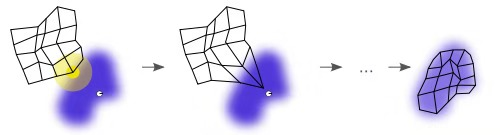
\includegraphics[width=2.2in]{./figs/SOM3.png}
\caption{ Hexagonal}
\end{minipage}
\end{figure}
\end{frame}



\begin{frame}{Details}

\begin{equation*}
f_{i+1}(N)=f_i(N)+\tau(d(N,N_p),i)(P-f_i(N))
\end{equation*}
The learning rate $\tau$ is define by $\tau(x,i)=0.02T/(T+100i)$ for $x=\rho(i)$, where $i$ is iteration number i and $T$ is the maximum number of iterations. $\tau$ decreases with distance of node $N$ from $N_p$
and with iteration number $i$. $P$ is data point.
\end{frame}


\begin{frame}{Details}
\begin{figure}[htbp]
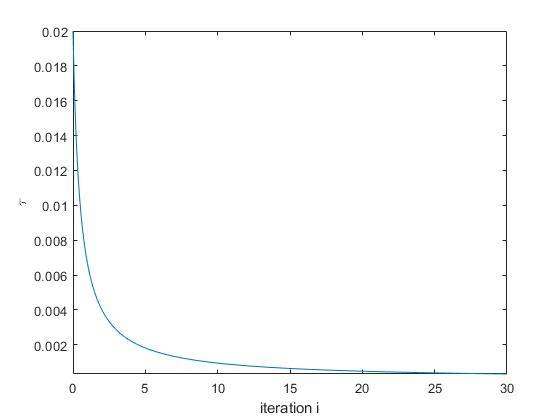
\includegraphics[width=8cm]{./figs/tau.jpg}
\end{figure}
\begin{equation*}
\tau(x,i)=0.02T/(T+100i)
\end{equation*}
\end{frame}